\documentclass[a4paper, 11pt,oneside]{article}
\usepackage[utf8]{inputenc}
\usepackage[T1]{fontenc}
\usepackage[german]{babel}
\usepackage{amsmath}
\usepackage{amssymb}
\usepackage{graphicx}
\usepackage{float} % For [H] option for figures/tables
\usepackage{caption} % For captions
\usepackage{subcaption} % If subfigures are ever needed
\usepackage{geometry}
\geometry{a4paper, left=2.5cm, right=2.5cm, top=2.5cm, bottom=3cm} % Adjusted bottom margin for page numbers
\usepackage{array} % For better table column specifications, e.g., >{\centering\arraybackslash}m{3cm}
\usepackage{enumitem} % For customizing lists
\usepackage{setspace} % For line spacing if needed, e.g. \onehalfspacing
\usepackage{siunitx}
\sisetup{
	output-decimal-marker={,},
	per-mode=fraction,
	number-unit-product={~} % Non-breaking space between number and unit
}
\usepackage{booktabs} % For nicer tables (toprule, midrule, bottomrule)
\usepackage{hyperref}
\hypersetup{
	colorlinks=true,
	linkcolor=black, % Default black for links to match document style
	citecolor=black,
	filecolor=black,
	urlcolor=blue, % URLs can be blue
	pdftitle={Praktikum Elektrotechnik Versuch 1},
	pdfauthor={Felix Gaartz},
	pdfsubject={Elektrotechnik Praktikum},
	pdfkeywords={Einweggleichrichtung, Brückengleichrichtung, Siebschaltungen, Spannungsstabilisierung}
}

\usepackage{fancyhdr}
\pagestyle{fancy}
\fancyhf{} % Clear all header and footer fields
\fancyfoot[R]{\thepage} % Page number on the right side of the footer
\renewcommand{\headrulewidth}{0pt} % No header rule
\renewcommand{\footrulewidth}{0pt} % No footer rule

% University and Department information for the title page
\newcommand{\university}{HOCHSCHULE ALBSTADT-SIGMARINGEN}
\newcommand{\department}{STUDIENGANG TECHNISCHE INFORMATIK}

\begin{document}
	
	\begin{titlepage}
		\centering
		\vspace*{1cm}
		{\Large \textbf{\university}} \\
		\vspace*{0.5cm}
		{\Large \textbf{\department}} \\
		\vspace*{2.5cm}
		{\Huge \textbf{Praktikum Elektrotechnik}} \\
		\vspace*{1cm}
		{\LARGE Versuch 1} \\
		\begin{center}
			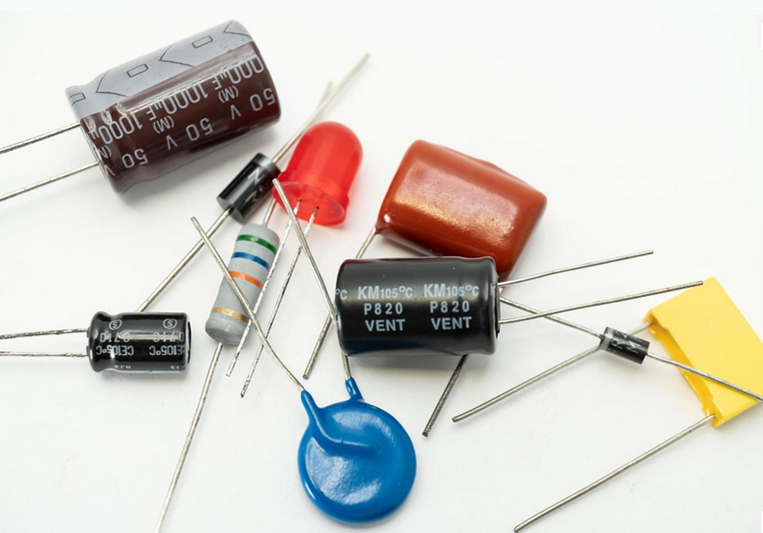
\includegraphics[width=0.7\linewidth]{screenshot012}
		\end{center}
		
		{\Large Gruppe 2} \\
		\vspace*{0.5cm}
		{\large Felix Gaartz} \\
		\vfill
		{\large \today}
	\end{titlepage}
	
	\newpage
	\tableofcontents
	\newpage
	
	\section{Einweggleichrichtung}
	
	\subsection{Einweggleichrichtung mit ohmscher Belastung ohne Kondensator}
	
	\textbf{Messaufbau:}
	\begin{itemize}
		\item 1 Widerstand $R=\SI{1}{\kilo\ohm}$
		\item 1 Widerstand $R_{m}=\SI{10}{\ohm}$
		\item 1 Diode V1, Typ 1N4001
	\end{itemize}
	
\begin{center}
	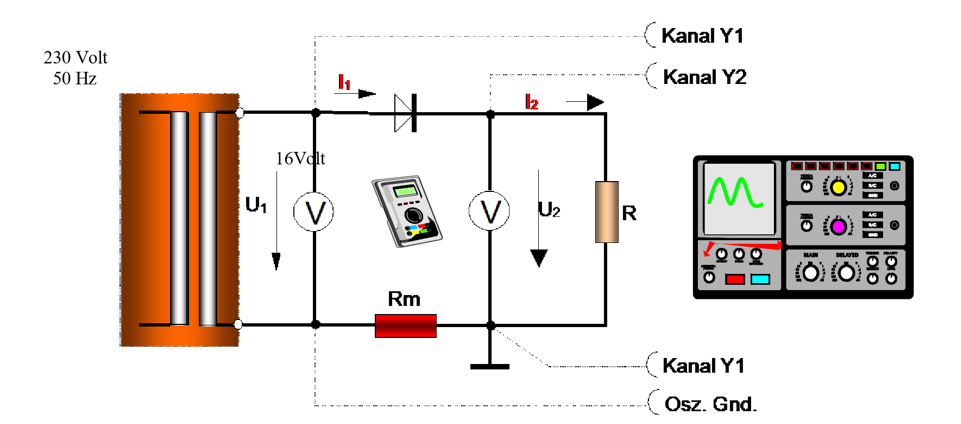
\includegraphics[width=0.8\textwidth]{screenshot001}
\end{center}
	
	\subsubsection{Messaufgaben}
	
	\textbf{Messaufgabe 1}
	
	\textit{Aufgabe:} Skizzieren Sie die Spannungs- und Stromverläufe $U_{1}(t)$, $U_{2}(t)$ und $I_{1}(t)$.
	
	\textit{Durchführung:} Schaltung aufbauen. $U_{1}=\SI{16}{V}$ einstellen mit Regler am roten Netztrafo. Oszillograph anschließen. Messen Sie den Diodenstrom $I_{D}(t)$ indirekt am Messwiderstand $R_{m}$.
	
\begin{center}
	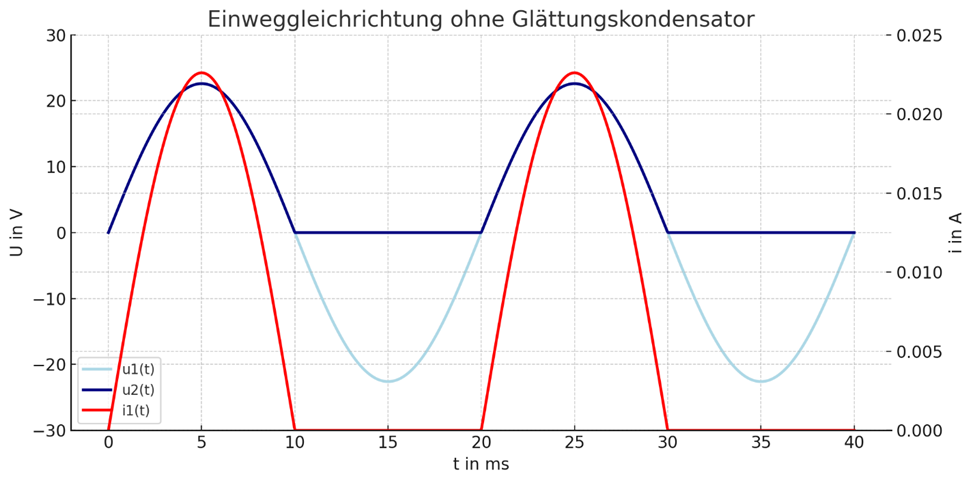
\includegraphics[width=\textwidth]{screenshot002}
\end{center}
	
	\textbf{Messaufgabe 2}
	
	\textit{Aufgabe:} Messen sie mit dem Oszillograph und Multimeter.
	
	\subsubsection{Auswertung}
	
	\begin{table}[H]
		\centering
		\caption{Messergebnisse Einweggleichrichtung ohne Kondensator}
		\label{tab:mess_einweg_ohne_k}
		\begin{tabular}{l l l}
			\toprule
			Messgröße & Symbol & Messergebnis \\
			\midrule
			Frequenz der Eingangsspannung & $f$ & \SI{50}{Hz} \\
			Brummspannungsfrequenz & $f_{br}$ & \SI{50}{Hz} \\
			Scheitelwerte & $U_{1_{max}}$ & \SI{-22,5}{V} -- \SI{22,5}{V} \\
			Scheitelwert & $U_{2_{max}}$ & \SI{0}{V} -- \SI{21}{V} \\
			Stromflusswinkel & $\alpha [\si{\degree}]$ & \SI{0}{\degree} \\
			Brummspannung & $U_{brmax}$ & \SI{21,3}{V} \\
			Effektivwert & $U_{1}$ & \SI{16,06}{V} \\
			Gleichspannung & $U_{2-}$ & \SI{6,84}{V} \\
			\bottomrule
		\end{tabular}
	\end{table}
	
	\textbf{Aufgabe 1:} Berechnen Sie aus den Messwerten das Verhältnis $\frac{U_{1}}{U_{2-}}$. Geben Sie den gemessenen und den theoretischen Wert an (mit Herleitung).
	
	Aus den Messwerten errechnet:
	$$ \frac{U_{1}}{U_{2-}}=\frac{\SI{16,06}{V}}{\SI{6,84}{V}}\approx2,35 $$
	
	Theoretisch gilt:
	$$ U_{2-}=\frac{U_{1}}{\sqrt{2}} $$
	Daraus folgt:
	$$ \frac{U_{1}}{U_{2-}}=\frac{U_{1}}{\frac{U_{1}}{\sqrt{2}}}=\sqrt{2}\approx1,4141 $$
	
	\textbf{Aufgabe 2:} Erklären Sie die indirekte Strommessung mit dem Oszillograph, und geben Sie den gemessenen und errechneten Wert an. Begründen Sie den Unterschied zwischen den Werten.\\
	
	$I_{gemessen}=\SI{22,00}{mA}$
	
	$I_{errechnet}=\SI{21,08}{mA}$\\
	
	Da der Strom I innerhalb des Schaltkreises gleich groß ist, lässt er sich über den Spannungsabfall an einem Widerstand errechnen. In unserem Fall haben wir mit dem Oszillograph am Messwiderstand die Spannung $U_{R_{m}}=\SI{220}{mV}$ gemessen. Damit lässt sich jetzt der Strom folgendermaßen berechnen:
	$$ I_{gemessen}=\frac{U_{R_{m}}}{R_{m}} $$
	$$ I_{gemessen}=\frac{\SI{0,22}{V}}{\SI{10}{\ohm}} $$ % Korrigiert von 22V zu 0.22V basierend auf Text und Ergebnis
	$$ I_{gemessen}=\SI{22}{mA} $$
	Um den Strom ohne eine Messung zu berechnen, benötigen wir die folgenden Größen:
	\begin{itemize}
		\item den Gesamtwiderstand der Schaltung $R_{ges}$
		\item Spannungsabfall der gesamten Schaltung $U_{ges}=U_{1}$
	\end{itemize}
	Der Gesamtwiderstand $R_{ges}$ setzt sich aus den Einzelwiderständen in der Schaltung zusammen:
	$$ R_{ges}=R+R_{m}=\SI{1000}{\ohm} + \SI{10}{\ohm} = \SI{1010}{\ohm} $$
	Mit $R_{ges}=\SI{1010}{\ohm}$ und $U_{ges}=U_{1}=\SI{22}{V}$ (Scheitelwert):
	$$ I_{berechnet}=\frac{U_{ges}}{R_{ges}} $$
	$$ I_{berechnet}=\frac{\SI{22}{V}}{\SI{1010}{\ohm}} $$
	$$ I_{berechnet}\approx\SI{21,7}{mA} $$
	Der Unterschied zwischen den beiden Werten entsteht durch Messfehler und Toleranzen bei den Widerständen. Die Widerstände dürfen eine 10\%-ige Abweichung von ihrem angegebenen Wert besitzen. Bei einem Gesamtwiderstand von \SI{1010}{\ohm} sind \SI{0,63}{mA} innerhalb dieser Toleranz.
	
	\subsection{Einweggleichrichtung mit Glättungskondensator}
	
	\textbf{Messaufbau:}
	\begin{itemize}
		\item 1 Widerstand $R=\SI{1}{\kilo\ohm}$
		\item 1 Widerstand $R_{m}=\SI{10}{\ohm}$
		\item 1 Diode V1, Typ 1N4001
		\item 1 Kondensator $C=\SI{100}{\micro F}$, \SI{40}{V} Elektrolyt
	\end{itemize}
	
\begin{center}
	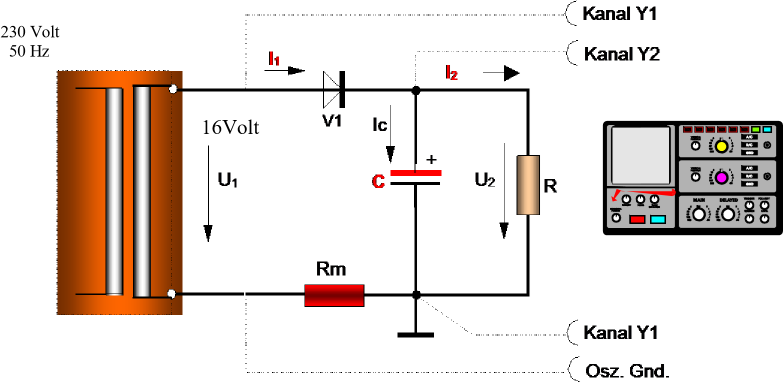
\includegraphics[width=0.8\textwidth]{screenshot011}
\end{center}
	
	\subsubsection{Messaufgaben}
	
	\textbf{Messaufgabe 1}
	
	\textit{Aufgabe:} Messen Sie die Spannungs- und Stromverläufe $U_{1}(t)$, $U_{2}(t)$, mit $I_{2}(t)=\frac{U_{2}(t)}{R}$ dem Oszillographen.
	
	\textit{Durchführung:} Schaltung aufbauen. $U_{1}=\SI{16}{V}$ einstellen.
	
\begin{center}
	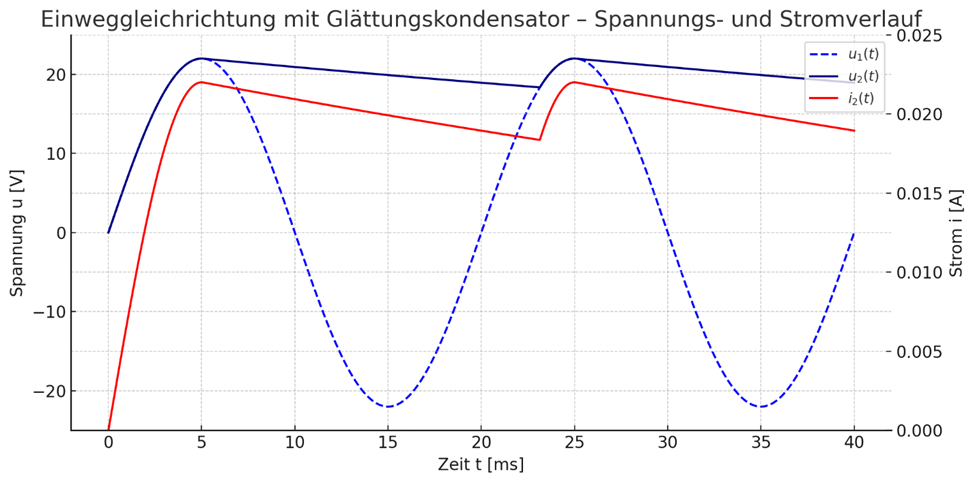
\includegraphics[width=\textwidth]{screenshot004}
\end{center}
	
	\textbf{Messaufgabe 2}
	
	\textit{Aufgabe:} Messen sie mit dem Oszillograph und Multimeter.
	
	\subsubsection{Auswertung}
	
	\begin{table}[H]
		\centering
		\caption{Messergebnisse Einweggleichrichtung mit Kondensator}
		\label{tab:mess_einweg_mit_k}
		\begin{tabular}{l l l}
			\toprule
			Messgröße & Symbol & Messergebnis \\
			\midrule
			Frequenz der Eingangsspannung & $f$ & \SI{50}{Hz} \\
			Brummspannungsfrequenz & $f_{br}$ & \SI{50}{Hz} \\
			Scheitelwerte & $U_{1_{max}}$ & \SI{-22,5}{V} -- \SI{22,5}{V} \\
			Scheitelwert & $U_{2_{max}}$ & \SI{21}{V} \\
			Stromflusswinkel & $\alpha [\si{\degree}]$ & \SI{0}{\degree} \\
			Brummspannung & $U_{brmax}$ & \SI{4}{V} \\
			Effektivwert & $U_{1}$ & \SI{16,04}{V} \\
			Gleichspannung & $U_{2}$ & \SI{19,18}{V} \\ % U2 statt U2-
			\bottomrule
		\end{tabular}
	\end{table}
	
	\textbf{Aufgabe 1:} Bestätigen Sie die Näherung $U_{2}\approx\sqrt{2}\cdot(U_{1}-0,65)\cdot \cos(\frac{\alpha}{2})$.
	$$ U_{2}\approx\sqrt{2}\cdot(U_{1}-\SI{0,65}{V})\cdot \cos\left(\frac{\alpha}{2}\right) $$
	$$ \SI{21}{V}\approx\sqrt{2}\cdot(\SI{16,04}{V}-\SI{0,65}{V})\cdot \cos\left(\frac{\SI{0}{\degree}}{2}\right) $$
	$$ \SI{21}{V}\approx\sqrt{2}\cdot\SI{15,39}{V}\cdot1 $$
	$$ \SI{21}{V}\approx\SI{21,76}{V} $$
	
	\textbf{Aufgabe 2:} Bestimmen Sie den Glättungsfaktor G.
	$$ G=2\cdot\pi\cdot f\cdot C\cdot R $$
	mit Lastwiderstand $R=\SI{1}{\kilo\ohm}$, Kapazität des Glättungskondensator $C=\SI{100}{\micro F}$ und Frequenz der Eingangswechselspannung $f=\SI{50}{Hz}$.
	$$ G = 2\cdot\pi\cdot\SI{50}{Hz}\cdot\SI{100}{\micro F}\cdot\SI{1}{\kilo\ohm} $$
	$$ G = 2\cdot3,14\cdot\SI{50}{Hz}\cdot\SI{100e-6}{F}\cdot\SI{1010}{\ohm} $$
	$$ G = 31,73 $$
	
	\section{Brückengleichrichtung}
	
	\subsection{Brückengleichrichtung ohne Glättungskondensator}
	
	\textbf{Messaufbau:}
	\begin{itemize}
		\item 1 Widerstand $R=\SI{1}{\kilo\ohm}$
		\item 1 Widerstand $R_{m}=\SI{10}{\ohm}$
		\item Brückengleichrichter Typ B80 C 1000/1500
	\end{itemize}
	
\begin{center}
	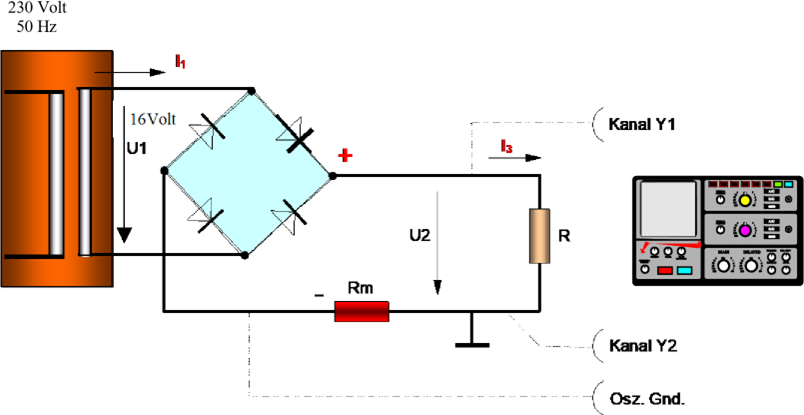
\includegraphics[width=0.8\textwidth]{screenshot005}
\end{center}
	
	\subsubsection{Messaufgaben}
	
	\textbf{Messaufgabe 1}
	
	\textit{Aufgabe:} Zeichnen Sie die Spannungs- und Stromverläufe $U_1(t)$, $U_2(t)$ und $I_2(t)$ auf.
	
	\textit{Durchführung:} Schaltung aufbauen. $U_1 = \SI{16}{V}$ einstellen. Oszillograph anschließen.
	
\begin{center}
	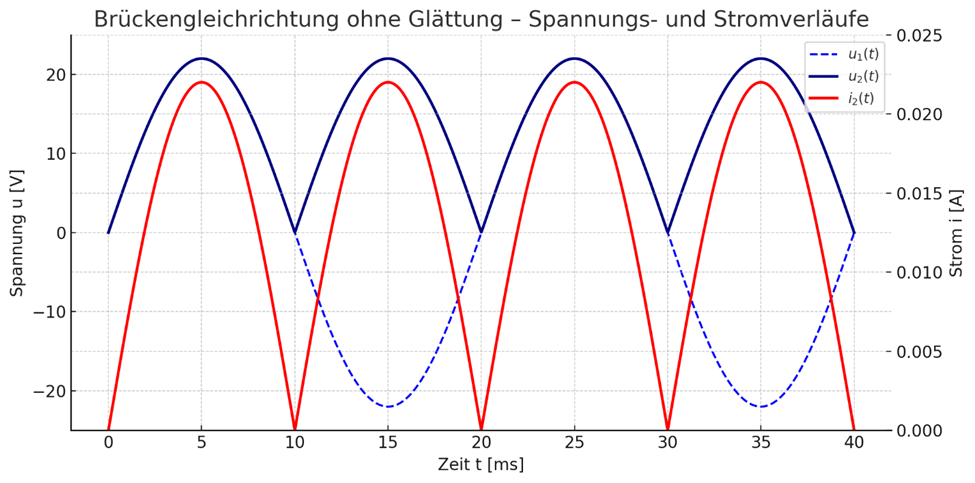
\includegraphics[width=\textwidth]{screenshot006}
\end{center}
	
	\textbf{Messaufgabe 2}
	
	\textit{Aufgabe:} Messen sie mit dem Oszillograph und Multimeter.
	
	\subsubsection{Auswertung}
	
	\textbf{Aufgabe 1:} Berechnen Sie aus den Messwerten das Verhältnis $\frac{U_1}{U_{2-}}$. Geben Sie den theoretischen Wert an (Herleitung, Diodenspannung vernachlässigt).
	
	Aus den Messwerten errechnet:
	$$ \frac{U_1}{U_{2-}} = \frac{\SI{16,01}{V}}{\SI{12,97}{V}} = 1,234 $$
	
	\begin{table}[H]
		\centering
		\caption{Messergebnisse Brückengleichrichtung ohne Glättungskondensator}
		\label{tab:mess_bruecke_ohne_k}
		\begin{tabular}{l l l}
			\toprule
			Messgröße & Symbol & Messergebnis \\
			\midrule
			Frequenz der Eingangsspannung & $f$ & \SI{50}{Hz} \\
			Brummspannungsfrequenz & $f_{br}$ & \SI{100}{Hz} \\
			Scheitelwerte & $U_{1max}$ & \SI{-22}{V} -- \SI{22}{V} \\
			Scheitelwert & $U_{2max}$ & \SI{0}{V} -- \SI{21}{V} \\
			Stromflusswinkel & $\alpha [\si{\degree}]$ & \SI{0}{\degree} \\
			Brummspannung & $U_{brmax}$ & \SI{21}{V} \\
			Effektivwert & $U_1$ & \SI{16,01}{V} \\
			Gleichspannung & $U_{2-}$ & \SI{12,97}{V} \\
			\bottomrule
		\end{tabular}
	\end{table}
	
	Theoretisch:
	$$ U_{2-} = \sqrt{2} \cdot U_1 \cdot \cos\left(\frac{\alpha}{2}\right) \approx \sqrt{2} \cdot U_1 \cdot \cos\left(\frac{\SI{0}{\degree}}{2}\right) \approx \sqrt{2} \cdot U_1 \cdot 1 $$
	Damit:
	$$ \frac{U_1}{U_{2-}} = \frac{U_1}{\sqrt{2} \cdot U_1} = \frac{1}{\sqrt{2}} \approx 0,707 $$
	
	\subsection{Brückengleichrichtung mit Glättungskondensator}
	
	\textbf{Messaufbau:}
	\begin{itemize}
		\item 1 Widerstand $R = \SI{1}{\kilo\ohm}$
		\item 1 Widerstand $R_m = \SI{10}{\ohm}$
		\item 1 Kondensator $C = \SI{33}{\micro F}$, \SI{40}{V}
		\item 1 Kondensator $C = \SI{100}{\micro F}$, \SI{40}{V}
		\item 1 Kondensator $C = \SI{220}{\micro F}$, \SI{40}{V}
		\item 1 Kondensator $C = \SI{1000}{\micro F}$, \SI{40}{V}
		\item Brückengleichrichter Typ B80 C 1000/1500
	\end{itemize}
	
\begin{center}
	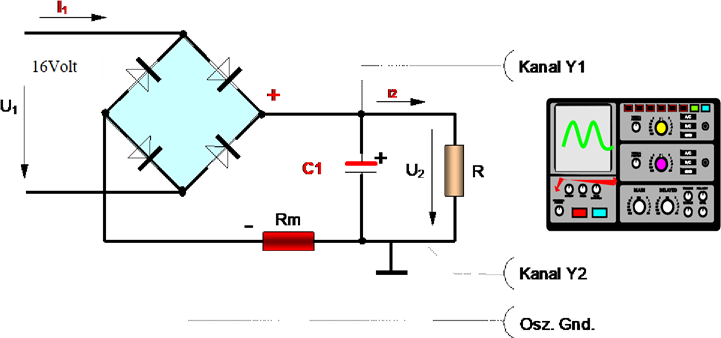
\includegraphics[width=0.8\textwidth]{screenshot007}
\end{center}
	
	\subsubsection{Messaufgaben}
	
	\textbf{Messaufgabe 1}
	
	\textit{Aufgabe:} Messen und skizzieren Sie für $C$ mit $\SI{33}{\micro F}$ die Spannungs- und Stromverläufe von $U_2(t)$ und $I_2(t)$ auf.
	
	\textit{Durchführung:} Schaltung aufbauen. $U_1 = \SI{16}{V}$ einstellen. Werte messen und aufschreiben.
	$$U_2 = \SI{18,55}{V}$$
	$$I_2 = \frac{\SI{18,55}{V}}{\SI{1}{\kilo\ohm}} = \SI{18,55}{mA}$$
	
\begin{center}
	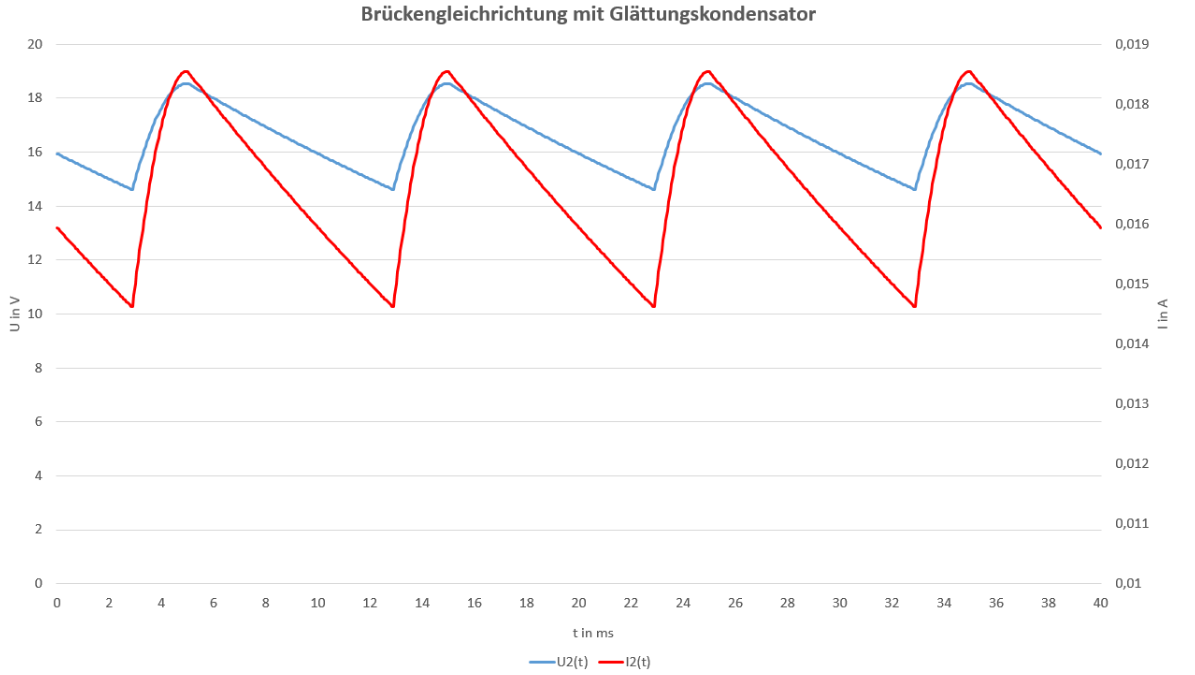
\includegraphics[width=\textwidth]{screenshot008}
\end{center}
	
	\textbf{Messaufgabe 2}
	
	\textit{Aufgabe:} Protokollieren Sie die Werte für verschiedene Größen des Kondensators $C_1$ in u.a. Tabelle. (Setzen Sie abwechseln die verschiedenen Kondensatoren in die Schaltung ein).
	

	\begin{table}[H]
		\centering
		\caption{Messwertetabelle Brückengleichrichtung mit Glättungskondensator}
		\label{tab:mess_bruecke_mit_k_varianten}
		\begin{tabular}{l c c c c }
			\toprule
			$C [\si{\micro F}]$ & {33} & {100} & {220} & {1000} \\
			\midrule
			$f_{Eingang} [\si{Hz}]$ & 50 & 50 & 50 & 50 \\
			$f_{br} [\si{Hz}]$ & 100 & 100 & 100 & 100 \\
			$U_{brss} [\si{V}]$ & 4,4 & 1,9 & 1,4 & 1,1 \\
			$U_1/U_2$ & 1,186 & 1,126 & 1,119 & 1,119 \\
			$W (10^{-2})$ & 8,4 & 3,4 & 2,5 & 2,0 \\
			$U_1 [\si{V}]$ & 22 & 22 & 22 & 22 \\
			$U_2 [\si{V}]$ & 18,55 & 19,54 & 19,65 & 19,66 \\
			$G$ & 10,362 & 31,4 & 69,08 & 314 \\
			\bottomrule
		\end{tabular}
	\end{table}
	
	\subsubsection{Auswertung}
	
	\textbf{Aufgabe 1:} Berechnen Sie die Verhältnisse $\frac{U_1}{U_2}$, $W = \frac{U_{2w}}{U_2}$, sowie den Glättungsfaktor $G$ für obige Messreihe. Rechnen Sie mit $U_{2w} = \frac{U_{2brss}}{2,828}$. Beurteilen Sie die Ergebnisse in Bezug auf die Dimensionierung von Stromversorgungsschaltungen.\\
	
	Stromversorgungsschaltungen sollten immer einen Kondensator im Verhältnis $\frac{R_{Last}}{C} = \frac{1}{10^{-6}}$ besitzen.

	\section{Siebschaltungen}
	
	\subsection{RC-Siebung}
	
	\textbf{Messaufbau:}
	\begin{itemize}
		\item 1 Widerstand $R = \SI{470}{\ohm}$
		\item 1 Widerstand $R_s = ?$ \si{\ohm}
		\item 1 Kondensator $C_1 = \SI{22}{\micro F}$, \SI{40}{V}
		\item 1 Kondensator $C_s = ?$ \si{\micro F}, \SI{40}{V}
		\item Brückengleichrichter Typ B80 C 1000/1500
	\end{itemize}
	
\begin{center}
	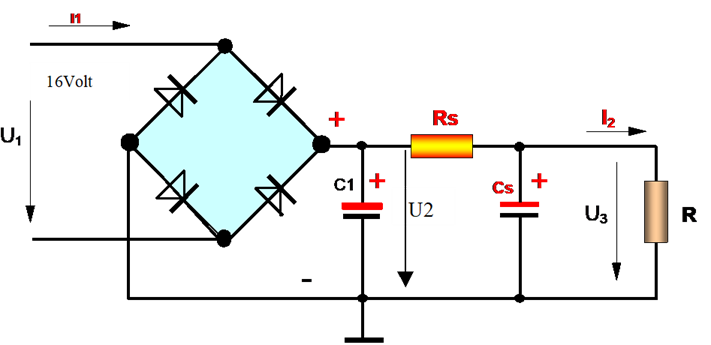
\includegraphics[width=0.8\textwidth]{screenshot009}
\end{center}
	
	\subsubsection{Messaufgaben}
	
	\textbf{Messaufgabe 1}
	
	\textit{Aufgabe:} Für die Gleichrichterschaltung aus 2.2 ist ein RC-Siebglied auszulegen. Dimensionieren Sie den Serienwiderstand $R_s$ (Widerstand, Leistung) und den Siebkondensator $C_s$ so, dass der Siebfaktor $s = \frac{U_{2w}}{U_{3w}}$ ca. 10 beträgt. Rechnen Sie mit der im Anhang angegebenen Näherungsformel für RC-Siebung. Folgende Randbedingungen sind einzuhalten: der zusätzliche Spannungsabfall am Serienwiderstand $R_s$ darf 10 \% der Ausgangsspannung (bei Nennstrom) nicht überschreiten. Maximale Ausgangslast $R = \SI{470}{\ohm}$. Messen Sie die Verhältnisse bei einer Belastung von $R = \SI{470}{\ohm}$ mit dem Oszillograph nach.
	
	\textit{Durchführung:} Schaltung aufbauen, Messwerte (Restwelligkeit) protokollieren und graphisch darstellen ($U_1,U_2,U_3$).
	
	\textit{Ergebnisse:} Die Näherung für den Siebfaktor lässt sich so umstellen, dass der Kondensator richtig gewählt werden kann. Als Widerstand wählen wir $\SI{47}{\ohm}$, damit haben wir 10 \% Spannungsabfall.
	$$ S = 2 \cdot \pi \cdot f_g \cdot C_s \cdot R_s \quad | \quad : (2 \cdot \pi \cdot f_g \cdot R_s) $$
	$$ C_s = \frac{S}{2 \cdot \pi \cdot f_g \cdot R_s} $$
	$$ C_s = \frac{10}{2 \cdot 3,14 \cdot \SI{100}{Hz} \cdot \SI{47}{\ohm}} $$
	$$ C_s = \SI{338}{\micro F} $$
	Spannungsverläufe:
\begin{center}
	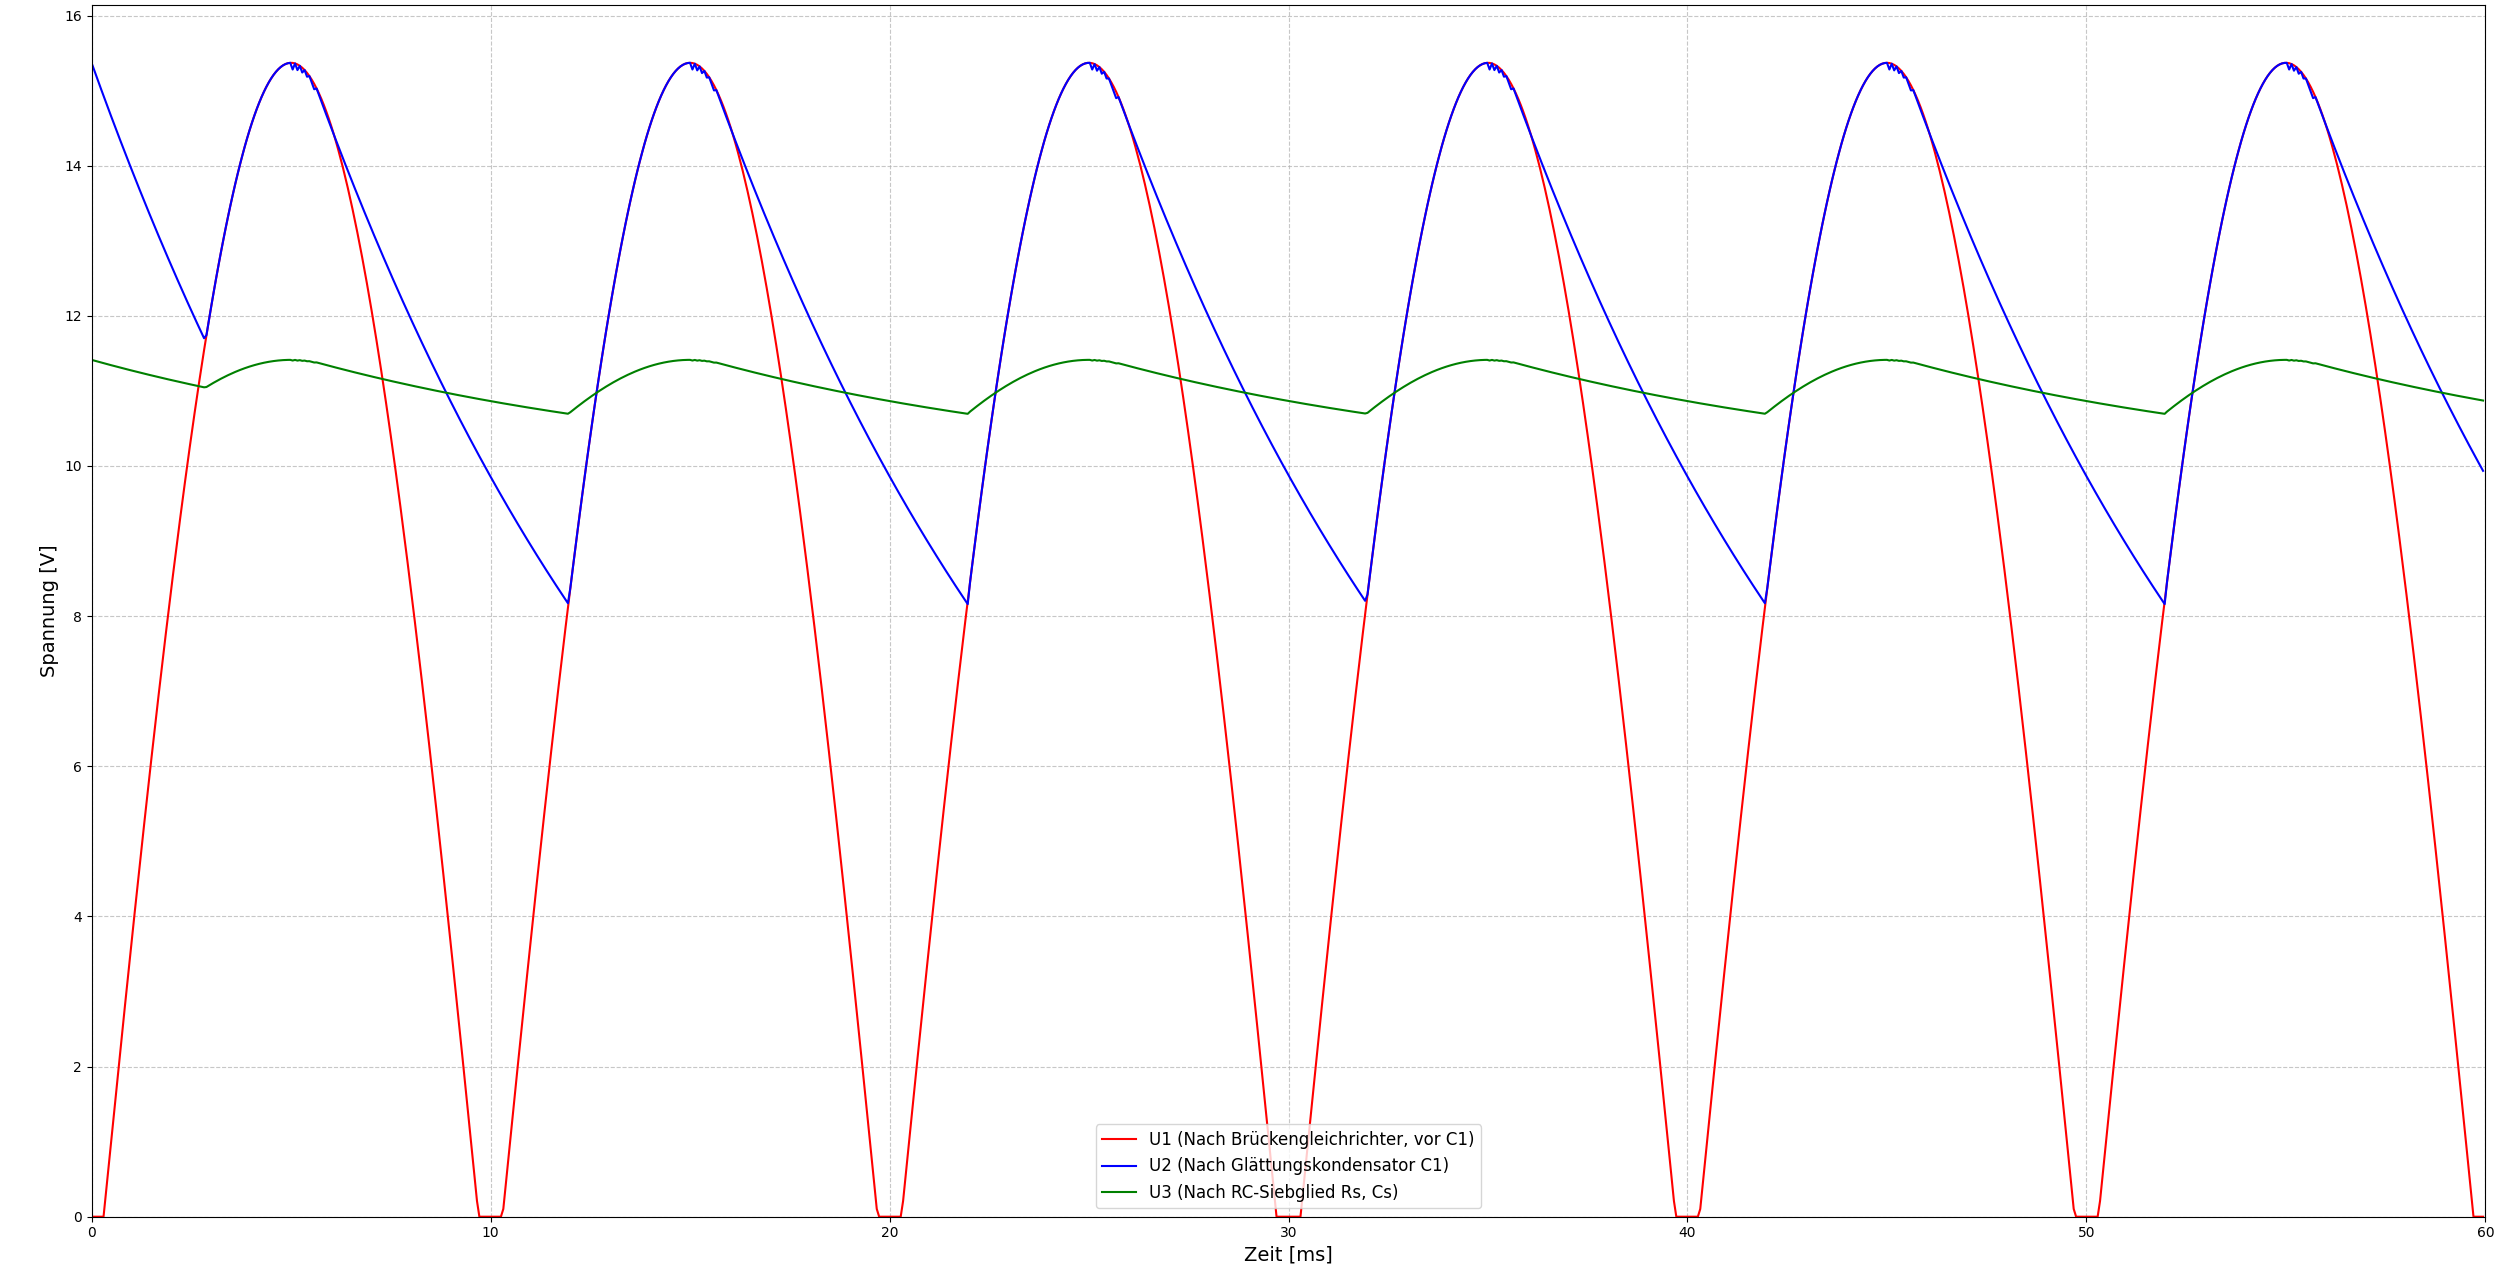
\includegraphics[width=1\linewidth]{screenshot013}
\end{center}

	
	
	\newpage
	\section{Spannungsstabilisierung}
	\subsection{Spannungsserienstabilisierung mit einem längsgeregeltem DC/DC-Wandler}
	
	\textbf{Messaufbau:}
	\begin{itemize}
		\item 1 Widerstand $R_{Last} = \SI{56}{\ohm}$, 10 \%, \SI{3}{W}
		\item 1 Widerstand $R_{Last} = \SI{220}{\ohm}$, 10 \%, \SI{3}{W}
		\item 1 Widerstand $R_{Last} = \SI{470}{\ohm}$, 10 \%, \SI{3}{W}
		\item 1 Widerstand $R_{Last} = \SI{1,2}{\kilo\ohm}$, 10 \%, \SI{3}{W}
		\item 1 Widerstand $R_1 = \SI{6,7}{\ohm}$, 10 \% 
		\item 1 Kondensator $C_1 = \SI{100}{\micro F}$, \SI{40}{V}
		\item 1 Kondensator $C_2 = \SI{22}{\micro F}$, \SI{40}{V}
		\item 1 Kondensator $C_3 = \SI{0,47}{\micro F}$, \SI{40}{V}
		\item Brückengleichrichter Typ B80 C 1000/1500
		\item Spannungsregler IC1, 7805
	\end{itemize}
	
\begin{center}
	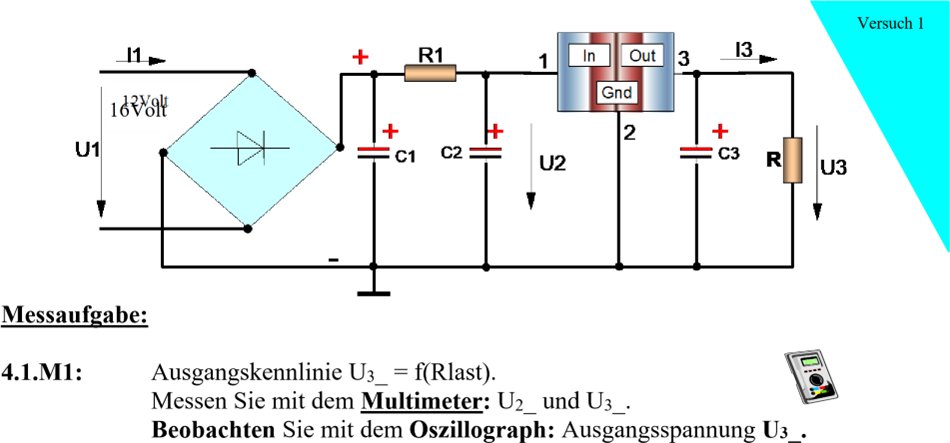
\includegraphics[width=0.8\textwidth]{screenshot010}
\end{center}
	
	\subsubsection{Messaufgaben}
	
	\textbf{Messaufgabe 1}
	
	\textit{Aufgabe:} Ausgangskennlinie $U_3 = f(R_{Last})$. Messen Sie mit dem Multimeter: $U_{2-}$ und $U_{3-}$. Beobachten Sie mit dem Oszillograph Ausgangsspannung $U_{3-}$.
	
	\textit{Durchführung:} Schaltung aufbauen. $U_1 = \SI{16}{V}$ einstellen. Messwerte für die verschiedenen Widerstände in die Tabelle 4.1 eintragen.
	
	\begin{table}[H]
		\centering
		\caption{Messwertetabelle Spannungsserienstabilisierung}
		\label{tab:spannung_stab}
		\begin{tabular}{l c c c c}
			\toprule
			$R_{Last} [\si{\ohm}]$ & {1200} & {470} & {220} & {56} \\
			\midrule
			$U_{2-} [\si{V}]$ & 20,29 & 20,06 & 19,62 & 17,56 \\
			$U_{3-} [\si{V}]$ & 4,97 & 4,97 & 4,97 & 4,95 \\
			$U_{3brss} [\si{mV}]$ & 4 & 5 & 7 & 16 \\
			$P_v [\si{W}]$ & 0,26 & 0,64 & 1,31 & 3,95 \\
			Wirkungsgrad in \% & 24,49 & 24,78 & 25,33 & 28,19 \\
			\bottomrule
		\end{tabular}
	\end{table}
	
	\textbf{Messaufgabe 2}
	
	\textit{Aufgabe:} Spannungsregler - Wirkungsgrad. Lastwiderstand $R_{Last} = \SI{100}{\ohm}$ Messen Sie mit dem Multimeter: $U_{2-}$ und $U_{3-}$, Werte notieren.
	
	\textit{Ergebnis:} Die Messung ergibt:
	$$U_{2-} = \SI{18,69}{V}$$
	$$U_{3-} = \SI{4,96}{V}$$
	
	\textbf{Messaufgabe 3}
	
	\textit{Aufgabe:} Ermitteln Sie die Eingangsspannung $U_1$ bei der die Schaltung für $R_{Last} = \SI{56}{\ohm}$ noch einwandfrei regelt und geben Sie den Spannungswert an. Beobachten Sie dazu die Ausgangsspannung $U_3(t)$ mit dem Oszillograph.
	
	\textit{Ergebnis:} Bei einer Eingangsspannung von $\SI{3,4}{V}$ regelt die Schaltung noch einwandfrei.
	
	\subsubsection{Auswertung}
	
	\textbf{Aufgabe 1:} Berechnen Sie zu allen Messwerten die Verlustleistung $P_v = P_{ce}$ und den Wirkungsgrad des Spannungsreglers (Eigenverbrauch vernachlässigt). Tragen Sie die Daten in die Tabelle 4.1 ein.
	
	Berechnung von $P_v$:
	$$ P_v = (U_2 - U_3) \cdot \frac{U_2}{R_{Last}} $$
	Berechnung des Wirkungsgrads $\eta$:
	$$ \eta = \frac{U_3}{U_2} $$
	
	
\end{document}